\documentclass[paper=a4, english]{article}

\usepackage[T1]{fontenc}
\usepackage[utf8]{inputenc}
\usepackage{fourier}
\usepackage{geometry}
\geometry{verbose,tmargin=2.5cm,bmargin=2cm,lmargin=2.5cm,rmargin=2cm}
\usepackage{float}
\usepackage{textcomp}
\usepackage{amsmath}
\usepackage{stackrel}
\usepackage{graphicx}
\usepackage{esint}
\usepackage{tikz}
\usetikzlibrary{matrix,calc}

\makeatletter

\providecommand{\tabularnewline}{\\}

\usepackage{fancyhdr}
\usepackage{lscape}
\usepackage{amssymb}
\pagestyle{fancy}
\lhead{Electronica III - 22.13}
\chead{TPL1}
\rhead{ITBA}
\renewcommand{\headrulewidth}{1pt}
\renewcommand{\footrulewidth}{1pt}

\makeatother

\usepackage{babel}
\usepackage{tikz}
\usetikzlibrary{matrix,calc}

%isolated term
%#1 - Optional. Space between node and grouping line. Default=0
%#2 - node
%#3 - filling color
\newcommand{\implicantsol}[3][0]{
    \draw[rounded corners=3pt, fill=#3, opacity=0.3] ($(#2.north west)+(135:#1)$) rectangle ($(#2.south east)+(-45:#1)$);
    }


%internal group
%#1 - Optional. Space between node and grouping line. Default=0
%#2 - top left node
%#3 - bottom right node
%#4 - filling color
\newcommand{\implicant}[4][0]{
    \draw[rounded corners=3pt, fill=#4, opacity=0.3] ($(#2.north west)+(135:#1)$) rectangle ($(#3.south east)+(-45:#1)$);
    }

%group lateral borders
%#1 - Optional. Space between node and grouping line. Default=0
%#2 - top left node
%#3 - bottom right node
%#4 - filling color
\newcommand{\implicantcostats}[4][0]{
    \draw[rounded corners=3pt, fill=#4, opacity=0.3] ($(rf.east |- #2.north)+(90:#1)$)-| ($(#2.east)+(0:#1)$) |- ($(rf.east |- #3.south)+(-90:#1)$);
    \draw[rounded corners=3pt, fill=#4, opacity=0.3] ($(cf.west |- #2.north)+(90:#1)$) -| ($(#3.west)+(180:#1)$) |- ($(cf.west |- #3.south)+(-90:#1)$);
}

%group top-bottom borders
%#1 - Optional. Space between node and grouping line. Default=0
%#2 - top left node
%#3 - bottom right node
%#4 - filling color
\newcommand{\implicantdaltbaix}[4][0]{
    \draw[rounded corners=3pt, fill=#4, opacity=0.3] ($(cf.south -| #2.west)+(180:#1)$) |- ($(#2.south)+(-90:#1)$) -| ($(cf.south -| #3.east)+(0:#1)$);
    \draw[rounded corners=3pt, fill=#4, opacity=0.3] ($(rf.north -| #2.west)+(180:#1)$) |- ($(#3.north)+(90:#1)$) -| ($(rf.north -| #3.east)+(0:#1)$);
}

%group corners
%#1 - Optional. Space between node and grouping line. Default=0
%#2 - filling color
\newcommand{\implicantcantons}[2][0]{
    \draw[rounded corners=3pt, opacity=.3] ($(rf.east |- 0.south)+(-90:#1)$) -| ($(0.east |- cf.south)+(0:#1)$);
    \draw[rounded corners=3pt, opacity=.3] ($(rf.east |- 8.north)+(90:#1)$) -| ($(8.east |- rf.north)+(0:#1)$);
    \draw[rounded corners=3pt, opacity=.3] ($(cf.west |- 2.south)+(-90:#1)$) -| ($(2.west |- cf.south)+(180:#1)$);
    \draw[rounded corners=3pt, opacity=.3] ($(cf.west |- 10.north)+(90:#1)$) -| ($(10.west |- rf.north)+(180:#1)$);
    \fill[rounded corners=3pt, fill=#2, opacity=.3] ($(rf.east |- 0.south)+(-90:#1)$) -|  ($(0.east |- cf.south)+(0:#1)$) [sharp corners] ($(rf.east |- 0.south)+(-90:#1)$) |-  ($(0.east |- cf.south)+(0:#1)$) ;
    \fill[rounded corners=3pt, fill=#2, opacity=.3] ($(rf.east |- 8.north)+(90:#1)$) -| ($(8.east |- rf.north)+(0:#1)$) [sharp corners] ($(rf.east |- 8.north)+(90:#1)$) |- ($(8.east |- rf.north)+(0:#1)$) ;
    \fill[rounded corners=3pt, fill=#2, opacity=.3] ($(cf.west |- 2.south)+(-90:#1)$) -| ($(2.west |- cf.south)+(180:#1)$) [sharp corners]($(cf.west |- 2.south)+(-90:#1)$) |- ($(2.west |- cf.south)+(180:#1)$) ;
    \fill[rounded corners=3pt, fill=#2, opacity=.3] ($(cf.west |- 10.north)+(90:#1)$) -| ($(10.west |- rf.north)+(180:#1)$) [sharp corners] ($(cf.west |- 10.north)+(90:#1)$) |- ($(10.west |- rf.north)+(180:#1)$) ;
}

%Empty Karnaugh map 4x4
\newenvironment{Karnaugh}%
{
\begin{tikzpicture}[baseline=(current bounding box.north),scale=0.8]
\draw (0,0) grid (4,4);
\draw (0,4) -- node [pos=0.7,above right,anchor=south west] {cd} node [pos=0.7,below left,anchor=north east] {ab} ++(135:1);
%
\matrix (mapa) [matrix of nodes,
        column sep={0.8cm,between origins},
        row sep={0.8cm,between origins},
        every node/.style={minimum size=0.3mm},
        anchor=8.center,
        ampersand replacement=\&] at (0.5,0.5)
{
                       \& |(c00)| 00         \& |(c01)| 01         \& |(c11)| 11         \& |(c10)| 10         \& |(cf)| \phantom{00} \\
|(r00)| 00             \& |(0)|  \phantom{0} \& |(1)|  \phantom{0} \& |(3)|  \phantom{0} \& |(2)|  \phantom{0} \&                     \\
|(r01)| 01             \& |(4)|  \phantom{0} \& |(5)|  \phantom{0} \& |(7)|  \phantom{0} \& |(6)|  \phantom{0} \&                     \\
|(r11)| 11             \& |(12)| \phantom{0} \& |(13)| \phantom{0} \& |(15)| \phantom{0} \& |(14)| \phantom{0} \&                     \\
|(r10)| 10             \& |(8)|  \phantom{0} \& |(9)|  \phantom{0} \& |(11)| \phantom{0} \& |(10)| \phantom{0} \&                     \\
|(rf) | \phantom{00}   \&                    \&                    \&                    \&                    \&                     \\
};
}%
{
\end{tikzpicture}
}

%Empty Karnaugh map 2x4
\newenvironment{Karnaughvuit}%
{
\begin{tikzpicture}[baseline=(current bounding box.north),scale=0.8]
\draw (0,0) grid (4,2);
\draw (0,2) -- node [pos=0.7,above right,anchor=south west] {bc} node [pos=0.7,below left,anchor=north east] {a} ++(135:1);
%
\matrix (mapa) [matrix of nodes,
        column sep={0.8cm,between origins},
        row sep={0.8cm,between origins},
        every node/.style={minimum size=0.3mm},
        anchor=4.center,
        ampersand replacement=\&] at (0.5,0.5)
{
                      \& |(c00)| 00         \& |(c01)| 01         \& |(c11)| 11         \& |(c10)| 10         \& |(cf)| \phantom{00} \\
|(r00)| 0             \& |(0)|  \phantom{0} \& |(1)|  \phantom{0} \& |(3)|  \phantom{0} \& |(2)|  \phantom{0} \&                     \\
|(r01)| 1             \& |(4)|  \phantom{0} \& |(5)|  \phantom{0} \& |(7)|  \phantom{0} \& |(6)|  \phantom{0} \&                     \\
|(rf) | \phantom{00}  \&                    \&                    \&                    \&                    \&                     \\
};
}%
{
\end{tikzpicture}
}

%Empty Karnaugh map 2x2
\newenvironment{Karnaughquatre}%
{
\begin{tikzpicture}[baseline=(current bounding box.north),scale=0.8]
\draw (0,0) grid (2,2);
\draw (0,2) -- node [pos=0.7,above right,anchor=south west] {b} node [pos=0.7,below left,anchor=north east] {a} ++(135:1);
%
\matrix (mapa) [matrix of nodes,
        column sep={0.8cm,between origins},
        row sep={0.8cm,between origins},
        every node/.style={minimum size=0.3mm},
        anchor=2.center,
        ampersand replacement=\&] at (0.5,0.5)
{
          \& |(c00)| 0          \& |(c01)| 1  \\
|(r00)| 0 \& |(0)|  \phantom{0} \& |(1)|  \phantom{0} \\
|(r01)| 1 \& |(2)|  \phantom{0} \& |(3)|  \phantom{0} \\
};
}%
{
\end{tikzpicture}
}

%Defines 8 or 16 values (0,1,X)
\newcommand{\contingut}[1]{%
\foreach \x [count=\xi from 0]  in {#1}
     \path (\xi) node {\x};
}

%Places 1 in listed positions
\newcommand{\minterms}[1]{%
    \foreach \x in {#1}
        \path (\x) node {1};
}

%Places 0 in listed positions
\newcommand{\maxterms}[1]{%
    \foreach \x in {#1}
        \path (\x) node {0};
}

%Places X in listed positions
\newcommand{\indeterminats}[1]{%
    \foreach \x in {#1}
        \path (\x) node {X};
}

% \begin{document}
%     \begin{Karnaugh}
%         \contingut{0,0,0,0,0,0,0,0,0,0,0,0,0,0,0,0}
%        \implicant{0}{2}{red}
%        \implicant{5}{15}{purple}
%        \implicantdaltbaix[3pt]{3}{10}{blue}
%     \implicantcantons[2pt]{orange}
%        \implicantcostats{4}{14}{green}
%     \end{Karnaugh}
%     %
%     \begin{Karnaughvuit}
%        \minterms{3,4}
%         \maxterms{0,1,6,7}
%        \indeterminats{2,5}
%        \implicant{3}{2}{green}
%        \implicant{4}{5}{}
%     \end{Karnaughvuit}
%     %
%     \begin{Karnaughquatre}
%         \minterms{1,2}
%        \maxterms{0,3}
%        \implicantsol{1}{green}
%        \implicantsol{2}{red}
%     \end{Karnaughquatre}

% \end{document}

\newpage
\begin{document}
\section*{Task 4}
    In this case we need to convert a 4-bit number into its complement 
    to two. A truth table is built first with four outputs corresponding 
    to the four input bits of the number complemented, as shown below.
    \begin{table}[H]
        \begin{center}
        \begin{tabular}{|c|c|c|c||c|c|c|c|}
        \hline
        \multicolumn{4}{|c||}{4-Bit In} & \multicolumn{4}{|c|}{2-Comp. Out}
        \\ \hline
        $d$ & $c$ & $b$ & $a$ & $f_{d}$ & $f_{c}$ & $f_{b}$ & $f_{a}$\\
        \hline \hline
        0 & 0 & 0 & 0 & 0 & 0 & 0 & 0\\ \hline
        0 & 0 & 0 & 1 & 1 & 1 & 1 & 1\\ \hline
        0 & 0 & 1 & 0 & 1 & 1 & 1 & 0\\ \hline
        0 & 0 & 1 & 1 & 1 & 1 & 0 & 1\\ \hline
        0 & 1 & 0 & 0 & 1 & 1 & 0 & 0\\ \hline
        0 & 1 & 0 & 1 & 1 & 0 & 1 & 1\\ \hline
        0 & 1 & 1 & 0 & 1 & 0 & 1 & 0\\ \hline
        0 & 1 & 1 & 1 & 1 & 0 & 0 & 1\\ \hline
        1 & 0 & 0 & 0 & 1 & 0 & 0 & 0\\ \hline
        1 & 0 & 0 & 1 & 0 & 1 & 1 & 1\\ \hline
        1 & 0 & 1 & 0 & 0 & 1 & 1 & 0\\ \hline
        1 & 0 & 1 & 1 & 0 & 1 & 0 & 1\\ \hline
        1 & 1 & 0 & 0 & 0 & 1 & 0 & 0\\ \hline
        1 & 1 & 0 & 1 & 0 & 0 & 1 & 1\\ \hline
        1 & 1 & 1 & 0 & 0 & 0 & 1 & 0\\ \hline
        1 & 1 & 1 & 1 & 0 & 0 & 0 & 1\\ \hline
        \end{tabular}
        \caption{Outputs with complement to two.}
        \end{center}
        \end{table}
        \par
        The output functions are expressed based on the minternms.
        They are simplified using Karnaugh's Maps. Starting with $f_d$ function:\par
        \[
            f_{d}=\sum{(m_1,m_2,m_3,m_4,m_5,m_6,m_7,m_8)}
        \]
        \begin{centering}
            \begin{Karnaugh}
                \minterms{1,2,3,4,5,6,7,8}
                \maxterms{0,9,10,11,12,13,14,15}
                \implicantsol{8}{red}
                \implicant{4}{6}{red}
                \implicant{1}{3}{red}
                \implicant{2}{6}{blue}
            \end{Karnaugh}
        \par\end{centering}
        Solving the map with the indicated groups, the simplified 
        function remains as:
        \[
            \boxed{f_{d}=(d \cdot \overline{c} \cdot \overline{b} \cdot \overline{a})+
            (\overline{d} \cdot c)+(\overline{d} \cdot \overline{c} \cdot a)+
            (\overline{d} \cdot b \cdot \overline{a})}    
        \]
        \newpage
        Now, taking the $f_c$ function, we do the same:
        \[
            f_{c}=\sum{(m_1,m_2,m_3,m_4,m_9,m_{10},m_{11},m_{12})}
        \]
        \begin{centering}
            \begin{Karnaugh}
                \minterms{1,2,3,4,9,10,11,12}
                \maxterms{0,5,6,7,8,13,14,15}
                \implicant{4}{12}{red}
                \implicantdaltbaix{2}{10}{red}
                \implicantdaltbaix{1}{11}{red}
            \end{Karnaugh}
        \par\end{centering}
        With the indicated groups, we get the simplified funcion:
        \[
            \boxed{f_c=(c \cdot \overline{b} \cdot \overline{a})+
            (\overline{c} \cdot a)+
            (\overline{c} \cdot b \cdot \overline{a})}    
        \]\par
        Next, with the $f_b$ function:
        \[
            f_{b}=\sum{(m_1,m_2,m_5,m_6,m_9,m_{10},m_{13},m_{14})}    
        \]
        \begin{centering}
            \begin{Karnaugh}
                \minterms{1,5,13,9,2,6,14,10}
                \maxterms{0,4,12,8,3,7,15,11}
                \implicant{1}{9}{red}
                \implicant{2}{10}{red}
            \end{Karnaugh}
        \par\end{centering}
        Solving the map, we get:
        \[
            \boxed{f_b=(\overline{b} \cdot a)+(b \cdot \overline{a})}    
        \]\par
        For the last function $f_a$:
        \[
            f_{a}=\sum{m_1,m_3,m_5,m_7,m_9,m_{11},m_{13},m_{15}}    
        \]\par
        In the table it can be observed that the output depends 
        directly from input $a$. We can write the simplified 
        function without making the Karnaugh's map:
        \[
            \boxed{f_a=a}    
        \]
        \par
        Having already the four output functions, the implementation
        can be carried out in a circuit with AND, OR and NOT logic gates,
        as shown in the next page.
        \newpage
        \begin{figure}[H]
            \begin{centering}
            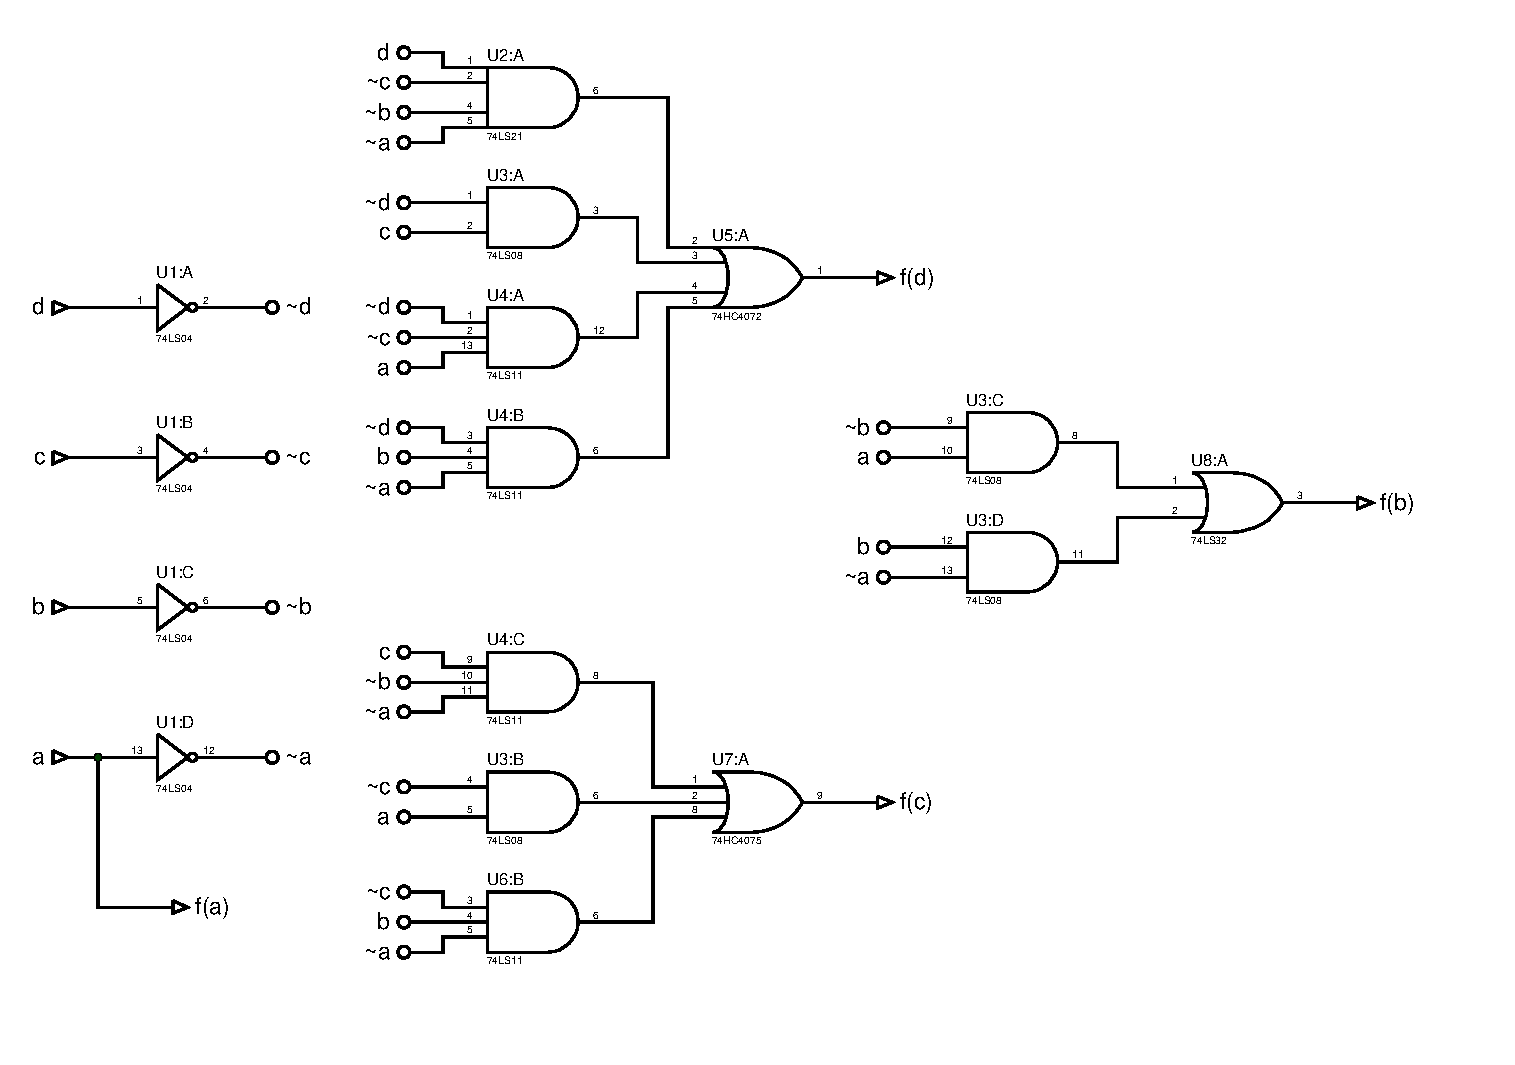
\includegraphics[width=1\textwidth]{data/ImplementacionEj4}
            \par\end{centering}
            \caption{Implementation of 2-complement circuit for a 4-bit input number - Designed in Proteus 7.8}
        \end{figure}
        
\end{document}
